%%% Local Variables:
%%% mode: latex
%%% TeX-master: "../main"
%%% coding: utf-8
%%% End:
% !TEX TS-program = pdflatexmk
% !TEX encoding = UTF-8 Unicode
% !TEX root = ../main.tex

As discussed in the introduction and theory chapters, the goal of this work is to implement a web-based path tracer. The path tracer is designed to be used for product visualization based on \gls{CAD} data, leveraging the \gls{OpenPBR} surface shading model.

The concrete result of this work consists of multiple parts. The report serves as the primary documentation of the work but does not contain all details. The library and code documentation is published under the \fGls{MIT license}{Permissive license originating at the Massachusetts Institute of Technology (MIT)} on GitHub with an accompanying website. See \url{https://www.github.com/StuckiSimon/strahl} for details. The library is published on the \fgls{npm}{package manager for JavaScript} registry as \texttt{strahl}. In addition, a dedicated short paper has been published for WEB3D '24: The 29th International ACM Conference on 3D Web Technology \cite{ownShortPaper}. The short paper includes the main insights and results of this work.

This section focuses on the implementation details of the path tracer. It also highlights the reasoning behind design decisions and provides insights into the performance of the renderer and its usability for the described use case.

For references to the implementation of the path tracer, a consistent notation is used. For example \coderef{ABC} refers to the code with the same comment. All relevant places are marked in code using the same reference, this permits using search features to find all references to a specific code section.

\section{Implementation}

The goal of the implementation is to be compatible with a large variety of devices and make the setup for consumers simple. Therefore, it is implemented and tested mainly in Chrome, which uses \gls{Dawn} as the underlying implementation of \gls{WebGPU}. Most notably, this means that dedicated features from other implementations such as \gls{wgpu} cannot be used. Neither can experimental extensions be leveraged.

The path tracer is designed to be integrated into existing web projects. The package is installable via \gls{npm}, but could also be downloaded and included manually. The full documentation is available on the website.

Figure~\ref{fig:path-tracer} illustrates the procedure of the path tracer. Scene preparation is performed on the CPU. This setup needs to be done once per visualization. Subsequent sampling of the scene is carried out repeatedly on the GPU, which constitutes the most computationally intensive part of the process.

\begin{figure}[H]
    \includegraphics[width=1.0\columnwidth]{resources/path-tracer-pipeline.png}
    \caption{Path Tracer Pipeline, distinguishing GPU and CPU tasks. The stages of the compute pipeline and render pipeline are executed sequentially.}
    \label{fig:path-tracer}
\end{figure}

\section{Scene Description}

In order to be easy to integrate for developers familiar with existing web-based rendering engines, the renderer utilizes many of the scene description constructs provided by \gls{Three.js}. This includes the representation of geometry using \texttt{BufferGeometry}, camera using \texttt{PerspectiveCamera}, and arbitrary camera controls such as \texttt{OrbitControls}.

This also enables to use a variety of loaders for different file formats such as \gls{OBJ} or \gls{glTF}. However, due to its advantages for transmission, it's advised to use the \gls{glTF} which can be imported using the loader provided by \gls{Three.js}.

\subsection*{Scene Preparation}

The main process involved with setting up the scene is the preparation of the \gls{BVH}. For \gls{BVH} construction, well-established solutions for the web are available. The path tracer uses \texttt{three-mesh-bvh} \cite{threeMeshBvh}. This method builds the \gls{BVH} on the \gls{CPU}, the code for transferring the \gls{BVH} to the \gls{GPU} is in \coderef{BVH-TRANSFER}.

In order to address memory alignment, as described in \autoref{ch:memoryAlignmentTheory}, the path tracer uses \texttt{webgpu-utils} \cite{webgpuUtilsLib}. The library enables a straightforward way to map data to buffers and align them correctly. See \coderef{MEMORY-VIEW} for creation of definition and \coderef{BUFFER-MAPPING} for mapping of data to buffers.

\todo{Memory Management (GPU+CPU)}

\section{Ray Generator}

The ray generator is responsible for casting rays into the scene according to the view projection. The path tracer employs a backward ray tracing approach, tracing rays from the camera into the scene.

\subsection*{View Projection}

For many applications, especially photorealistic rendering, perspective projection is used. Based on the assessed use cases, the path tracer uses perspective projection only. See \coderef{VIEWPROJECTION} for implementation.

\subsection*{Random Number Generator}

The path tracer uses PCG-RXS-M-XS variant as described by O’Neill \cite{o2014pcg} in combination with Xorshift as described by Marsaglia \cite{marsaglia2003xorshift}. See \coderef{RNG} for implementation.

In order to set up the Monte Carlo method, the \gls{RNG} needs to be employed in a suitable manner. As it is a pseudorandom generator, it necessitates a seed to start the generation. If the seed is identical for all pixels, the results of a single sample will frequently share similar patterns in adjacent surfaces as shown in \autoref{fig:rngBadSeed}. The result for independent seeds differs in a stark manner as shown in \autoref{fig:rngGoodSeed}.

\begin{figure}[H]
    \centering
    \begin{subfigure}[b]{0.45\textwidth}
        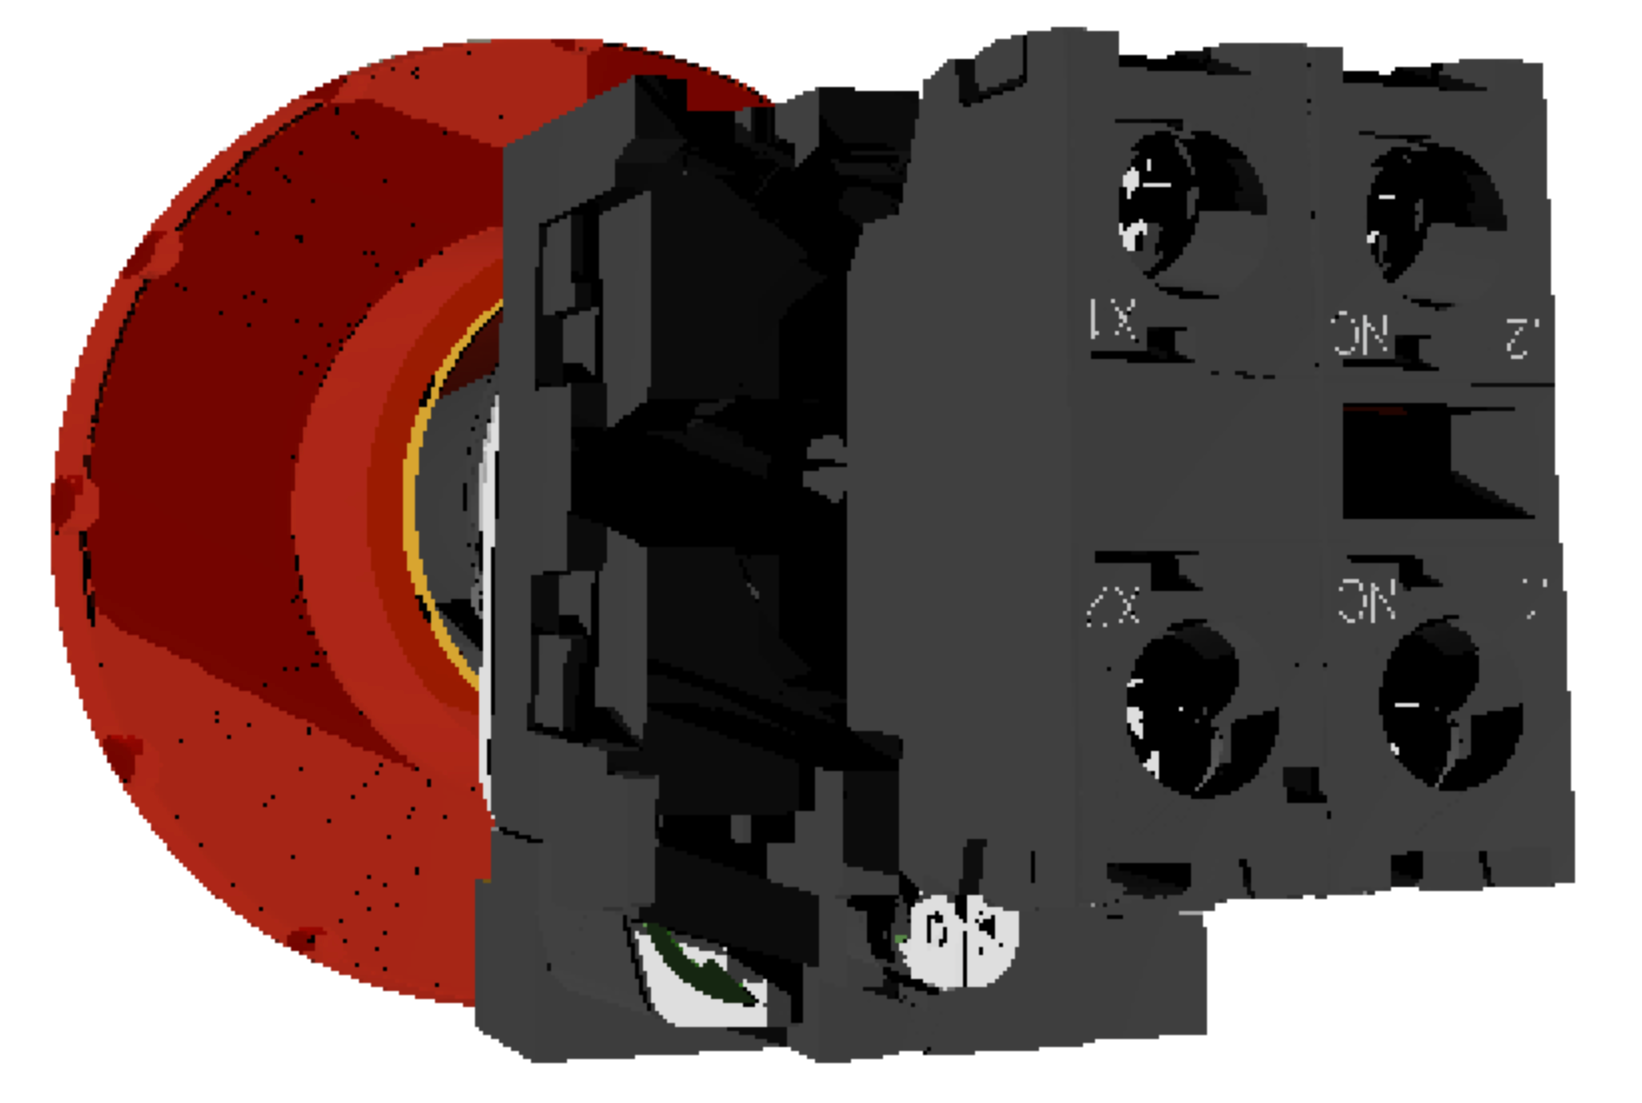
\includegraphics[width=\textwidth]{resources/single-sample-bad-seed.png}
        \caption{identical seed for all pixels}
        \label{fig:rngBadSeed}
    \end{subfigure}
    \hfill
    \begin{subfigure}[b]{0.45\textwidth}
        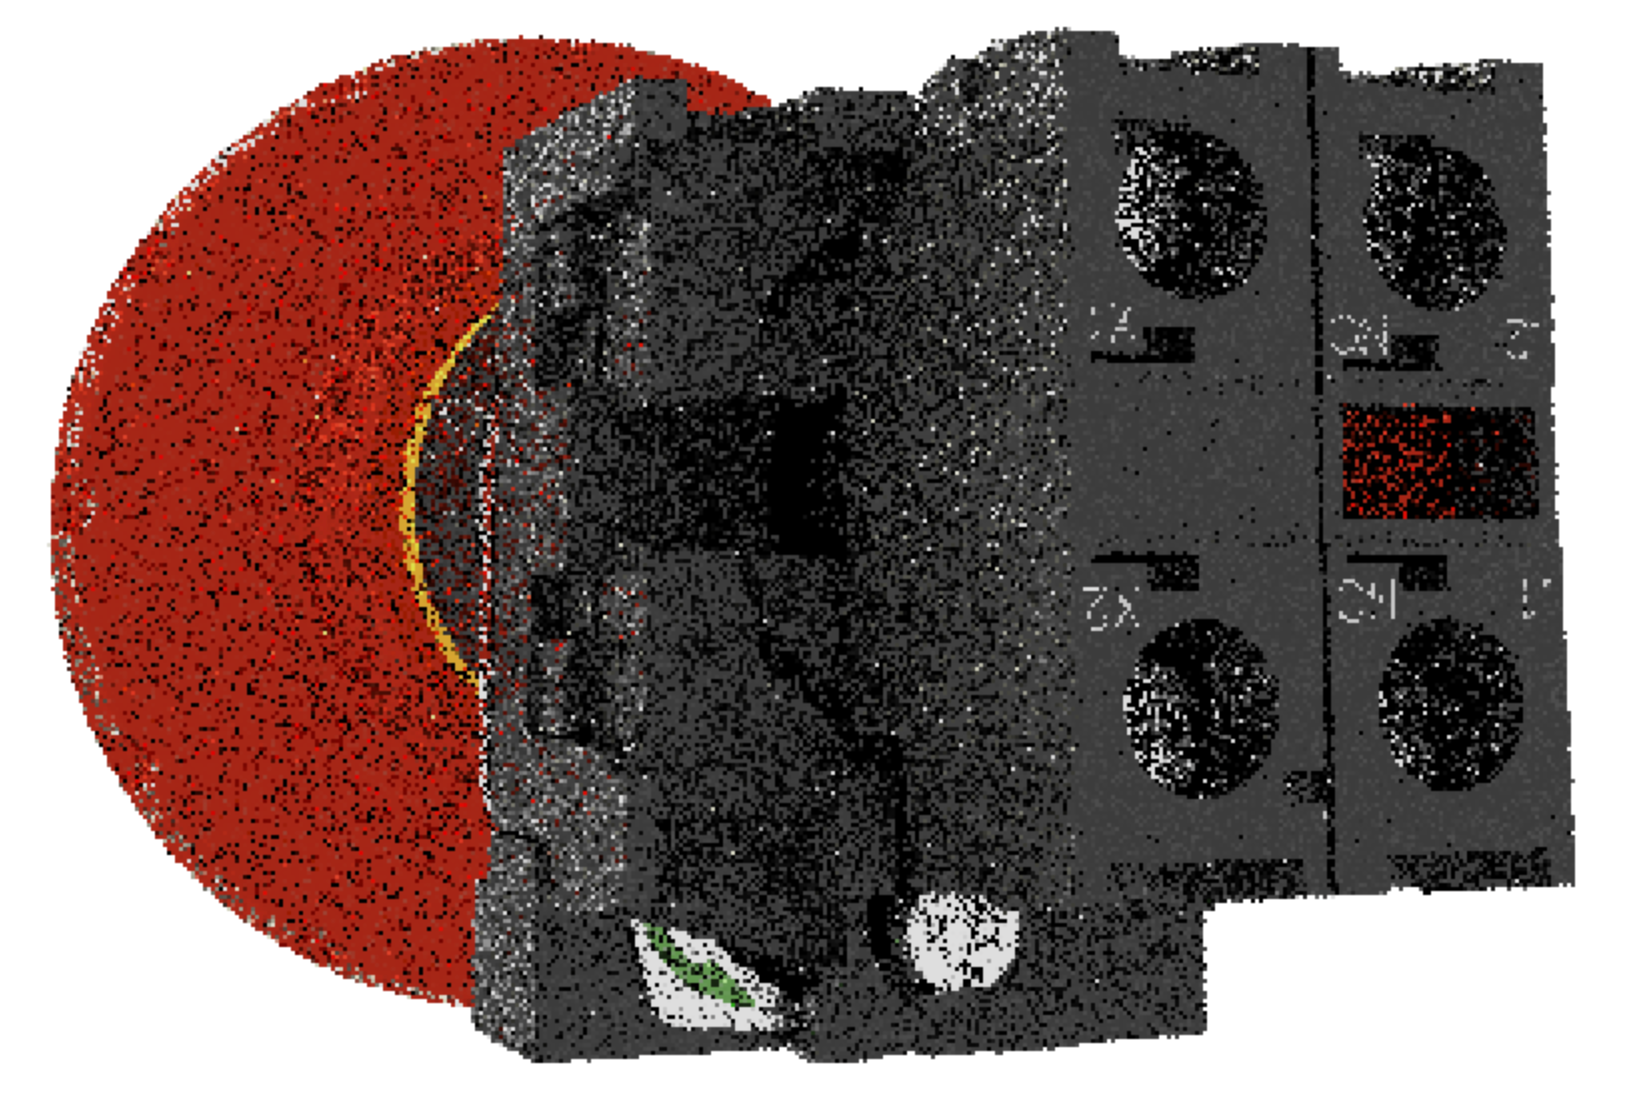
\includegraphics[width=\textwidth]{resources/single-sample-good-seed.png}
        \caption{independent seed for every pixel}
        \label{fig:rngGoodSeed}
    \end{subfigure}
    \caption{Both images consist of only one sample.}
    \label{fig:rngSeed}
\end{figure}

When increasing the sample count, the differences in the setup remain visible. Adjacent surfaces show similar patterns as shown in \autoref{fig:rngNoiseArtifactsHighlightsBadNoisy}, which resemble image compression artifacts encountered in aggressively compressed \fGlspl{JPEG}{\e{Joint Photographic Experts Group}, common method for lossy image compression}. In contrast, the renderings with independent seeds show stark differences in adjacent pixels akin to noise as shown in \autoref{fig:rngNoiseArtifactsHighlightsGoodNoisy}. As shown in \autoref{fig:rngNoiseArtifactsHighlightsBadAnti} compared to \autoref{fig:rngNoiseArtifactsHighlightsGoodAnti}, the anti-aliasing is less noticeable when using independent seeds.

\begin{figure}[H]
    \centering
    \hspace*{2cm}
    \begin{subfigure}[t]{0.3\textwidth}
        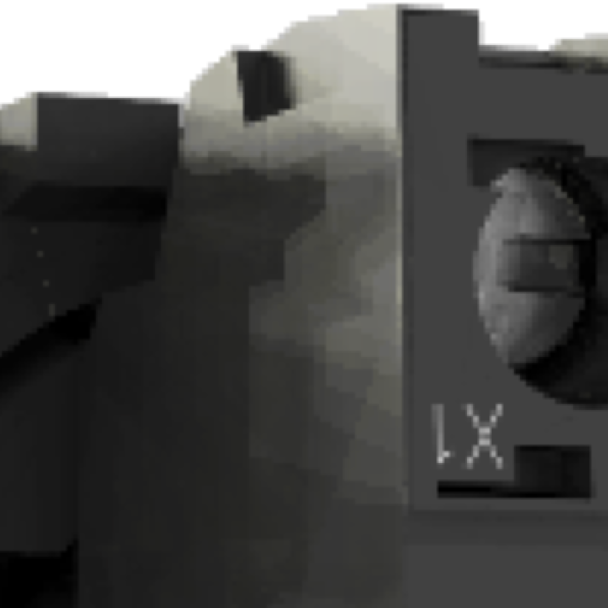
\includegraphics[width=\textwidth]{resources/bad-seed-noisy.png}
        \caption{Renderings which resemble lossy image compression artifacts.}
        \label{fig:rngNoiseArtifactsHighlightsBadNoisy}
    \end{subfigure}
    \hfill
    \begin{subfigure}[t]{0.3\textwidth}
        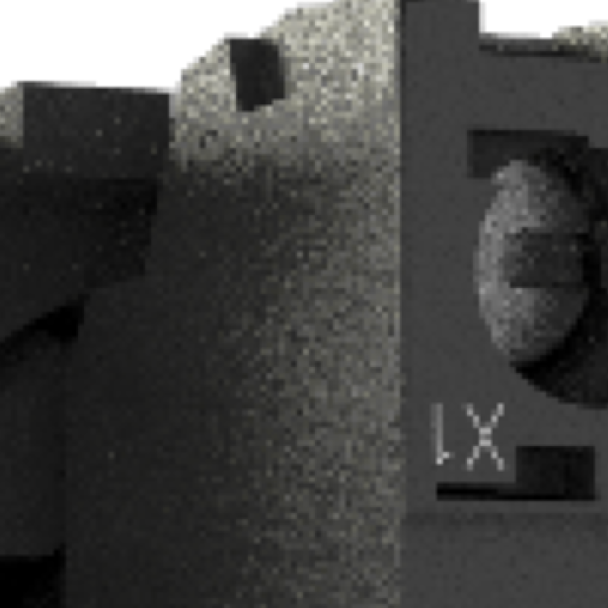
\includegraphics[width=\textwidth]{resources/good-seed-noisy.png}
        \caption{Noisy renderings with stark differences in adjacent pixels.}
        \label{fig:rngNoiseArtifactsHighlightsGoodNoisy}
    \end{subfigure}
    \hspace*{2cm}
    \vfill
    \vspace*{0.5cm}
    \hspace*{2cm}
    \begin{subfigure}[t]{0.3\textwidth}
        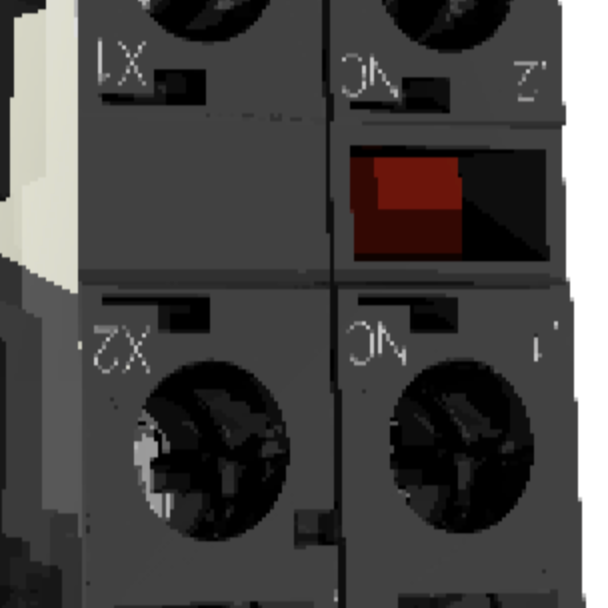
\includegraphics[width=\textwidth]{resources/bad-seed-anti-aliasing.png}
        \caption{On the right side, anti-aliasing is rather noticeable.}
        \label{fig:rngNoiseArtifactsHighlightsBadAnti}
    \end{subfigure}
    \hfill
    \begin{subfigure}[t]{0.3\textwidth}
        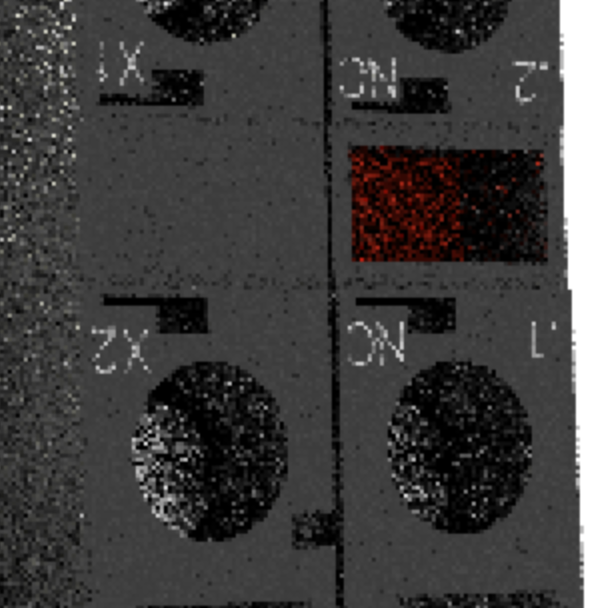
\includegraphics[width=\textwidth]{resources/good-seed-anti-aliasing.png}
        \caption{On the right side, anti-aliasing is less noticeable.}
        \label{fig:rngNoiseArtifactsHighlightsGoodAnti}
    \end{subfigure}
    \hspace*{2cm}
    \caption{Magnified images of renderings with low sample count showing difference based on seed setup. Left column has identical seed for all pixels of a sample, but varying seeds for different samples. Right column has independent seeds for every pixel of a sample as well as across samples.}
    \label{fig:rngNoiseArtifactsHighlights}
\end{figure}

\subsection*{Anti-Aliasing}
\label{sec:anti-aliasing-implementation}

The implementation of the strategy indicated in \ref{sec:anti-aliasing} is implemented in \coderef{ALIASING}.

\section{Path Tracer}

Intersection tests based on the \gls{BVH} are implemented in \gls{WGSL}, see \coderef{BVH-TESTS}. For each intersection, sampling is done according to the \gls{MIS} scheme.

The surface shading method is based on \gls{OpenPBR} reference implementation in \gls{MaterialX} as well as the reference viewer by Portsmouth \cite{openPbrViewer}.

The renderer uses \fGls{RGB}{\e{red, green, and blue}, common system for color representation in computer graphics} as the color space.

\section{Render Pipeline}

The output of the path tracing compute shader is a texture, which is then passed to a rasterizer. The rasterizer renders the texture to the canvas using a fullscreen quad consisting of two triangles. Tone mapping is done using the Khronos PBR Neutral Tone Mapper described in \autoref{sec:toneMappingTheory}. See \coderef{TONE-MAPPER} for implementation. Progressive rendering is a technique to render an image in multiple passes. Each render pass improves the quality of the image. This enables the user to see the rough image quickly and refine it over time. 

\section{Benchmark}
\label{sec:benchmark}

In order to assess the effectiveness of certain measures, a benchmark is defined to measure the performance of the path tracer. This benchmark is used for quantitative evaluation of the path tracer. Prior sections, such as anti-aliasing as described in \autoref{sec:anti-aliasing-implementation} focused on qualitative aspects of the path tracer. Depending on the use case, the benchmark can be adjusted to focus on different aspects. However, the core design of the benchmark remains the same. Generally, measurements are taken for the entirety of a stage instead of focusing on individual routines within a stage. This gives a more holistic view of the performance of the path tracer.

A total of 100 samples per pixel with a ray depth of five was used. The image was rendered in Chrome 126 at a resolution of 512$\times$512 pixels. Experiments were conducted with different model complexities. The simplified versions are decimated meshes of the original, which consists of roughly one million triangles. The LOD artifacts are shown in Figure~\ref{fig:benchmark-models}. The first two levels are intended to be visually similar, while the third level is a simplified version intended to demonstrate the effect of non-manifold geometry for ray tracing.

Unless otherwise specified, the benchmarks are conducted on a MacBook Pro with Apple Silicon M1 Max. The measurements were calculated using the mean time of 30 runs with a confidence interval of 95\% given as $\pm$ standard deviation from the mean time in milliseconds as discussed in \autoref{sec:probabilityTheory}.

\begin{figure}[H]
    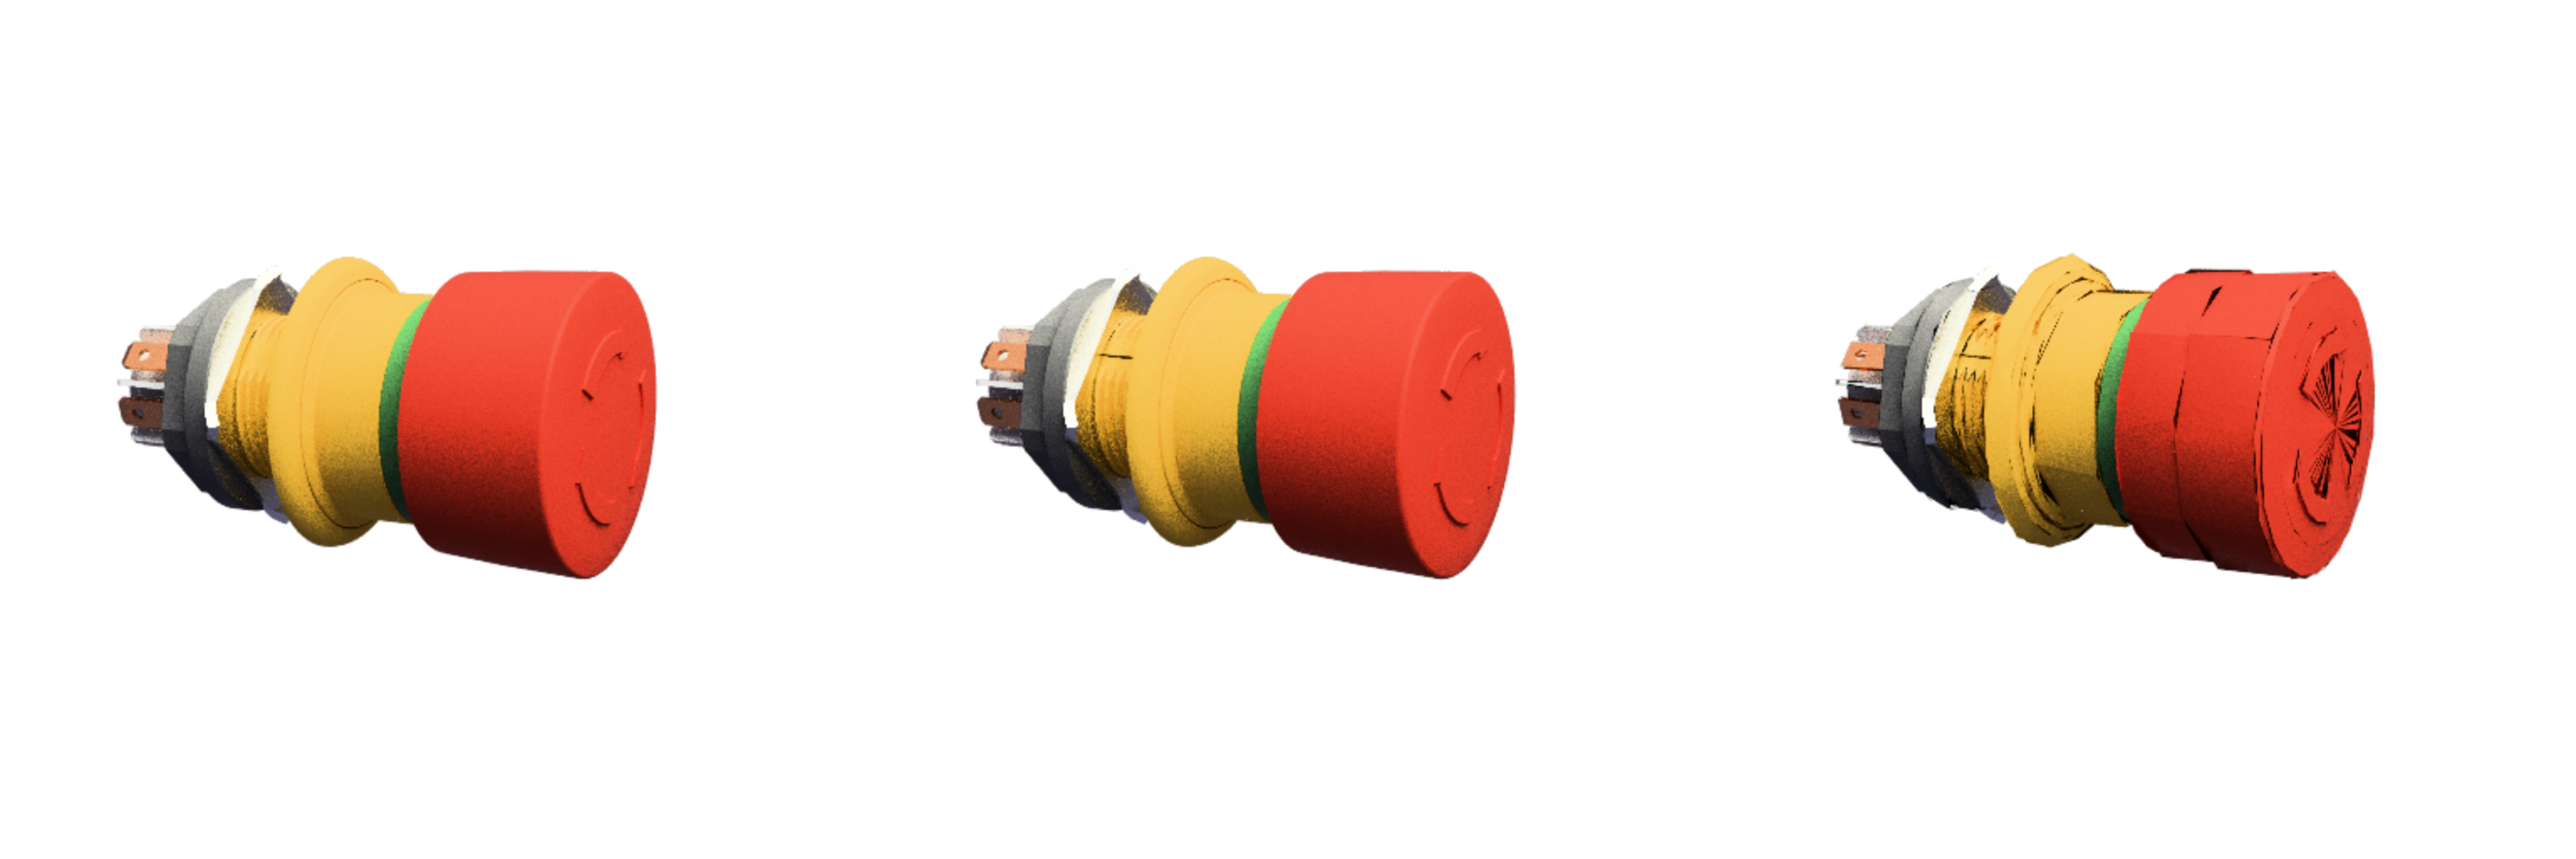
\includegraphics[width=0.9\columnwidth]{resources/benchmark-models.png}
    \caption{The three LOD artifacts and their short names in brackets, from left to right: 1,068,735 triangles (high), 106,873 triangles (mid), 10,687 triangles (low). The left and middle figures share similar visual fidelity characteristics.}
    \label{fig:benchmark-models}
\end{figure}

\subsection{Russian Roulette}

As described in \autoref{ch:russianRoulette}, Russian roulette is a technique used to do probabilistic path termination. The code is implemented in \coderef{RUSSIAN-ROULETTE}. The benchmark results are shown in \autoref{tab:russian-roulette-measurements}.

\begin{table}[H]
    \centering
    \ra{1.3}
    \begin{tabular}{@{}lll@{}}
    \toprule
    & With Russian roulette & Without Russian roulette \\
    High & 2361.77 ms $\pm$ 11.27 ms & 2583.40 ms $\pm$ 12.84 ms \\
    Mid & 2018.03 ms $\pm$ 8.76 ms & 2135.94 ms $\pm$ 8.14 ms \\
    Low & 2028.04 ms $\pm$ 10.78 ms & 2200.00 ms $\pm$ 8.91 ms \\
    \bottomrule
    \end{tabular}
    \caption{Benchmark results for Russian roulette optimization.}
    \label{tab:russian-roulette-measurements}
\end{table}

\subsection{Overall Performance}

The results for CPU performance were recorded using the Performance API and are presented in Table~\ref{tab:cpuPerformance}. The results for GPU performance were recorded using \gls{WebGPU} timestamp queries and are presented in Table~\ref{tab:gpuPerformance}. All measurements were calculated using the mean time of 30 benchmark samples, with a 95\% confidence interval given as $\pm$ standard deviation from the mean time in milliseconds.


\begin{table}[H]
  \centering
  \ra{1.3}
  \begin{tabular}{rrr}
    \toprule
    Triangles   & Apple M1 Max    & AMD/NVIDIA \\
    1,068,735     & 327.57 ms $\pm$ 0.56 ms     & 383.10 ms $\pm$ 4.06 ms \\
    106,873     & 45.49 ms $\pm$ 0.31 ms    & 41.77 ms $\pm$ 0.43 ms \\
    10,687     & 10.53 ms $\pm$ 0.24 ms    & 8.43 ms $\pm$ 0.22 ms \\
    \bottomrule
  \end{tabular}
  \caption{BVH setup time based on model complexity}
  \label{tab:cpuPerformance}
\end{table}

\begin{table}[H]
  \centering
  \ra{1.3}
  \begin{tabular}{rrr}
    \toprule
    Triangles   & Apple M1 Max    & AMD/NVIDIA \\
    1,068,735     & 2,319.45 ms $\pm$ 11.14 ms    & 1,058.73 ms $\pm$ 59.47 ms \\
    106,873     & 1,992.11 ms $\pm$ 8.49 ms    & 790.20 ms $\pm$ 3.79 ms\\
    10,687     & 2,031.38 ms $\pm$ 9.87 ms    & 790.83 ms $\pm$ 4.18 ms \\
    \bottomrule
  \end{tabular}
  \caption{GPU path tracer time based on model complexity}
  \label{tab:gpuPerformance}
\end{table}
  

\section{Use Case Scenarios}

The \gls{CAD} data used by EAO is a good fit for a path tracer. While not certain strengths of the ray tracing approach, such as caustics, are not relevant for the use case, and other strengths, such as reflections are not fully utilized, the path tracer still provides a suitable candidate for the use case. The complexity of the geometry does not pose a significant challenge for the path tracer, even for relatively high triangle counts. Using \gls{PBR} fits the use case and provides sufficient adjustment possibilities for the materials.

